%-----------------------------------------------------------------------------%
\chapter{\babSatu}
%-----------------------------------------------------------------------------%

This chapter explains the background of this research and the problem to be
solved by this research.

%-----------------------------------------------------------------------------%
\section{Research Background}
%-----------------------------------------------------------------------------%

In the early days of web development, every part of a web application was coded
manually. This required extensive knowledge of how the web works. Depending on
the web application, this might include understanding of the Hypertext Transfer
Protocol (HTTP), the Hypertext Markup Language (HTML), and other things such as
databases. If not done correctly, this could lead to a lot of errors and
security holes in the web application.

Web frameworks aim to solve this problem by providing a standard way to build
web applications. Web frameworks help eliminate the overhead of implementing
common parts of web applications such as the HTTP layer, the database layer,
and the view layer. This helps web developers build web applications more
quickly and safely by focusing more on the business logic of the web
application itself instead of the more intricate details.

Among the widely-used web frameworks is Django, a free and open-source web
framework written in Python \footnote{\url{https://djangoproject.com}}. One of
the main features of Django is an object-relational mapping (ORM) tool in the
database layer. The ORM tool maps data models, represented as Python classes,
to tables in a relational database. The columns of a database table are defined
as attributes (called fields) inside the model class \cite{django}.

While relational databases are useful in handling structured data, there has
been an increase in the popularity of non-relational databases, commonly known
as NoSQL databases \cite{paul_nosql}. NoSQL encourages the simplicity of
database design, which makes the process of scaling the database to multiple
clusters of machines easier \cite{leavitt_nosql}. NoSQL databases are also
considered as more flexible due to its dynamic schema.

However, NoSQL databases also have their own downsides. Most NoSQL databases
disregard the Atomicity, Consistency, Isolation, and Durability (ACID)
principles found in relational databases \cite{kyle_mongodb}. They also lack
the ability to perform joins across tables due to the use of denormalized data,
which makes it harder to deal with entity relations.

Nowadays, some relational database systems have come up with their own
solutions of providing a hybrid data model. This is done by combining
structured data with some form of semi-structured data, most commonly in
JavaScript Object Notation (JSON) format. This gives all the benefits of using
a relational database, while still allowing the simplicity and dynamic nature
of semi-structured data.

From version 1.9 until version 3.0, Django had provided an implementation of
JSONField. However, it was exclusively available for PostgreSQL. This JSONField
allowed its users to store and query JSON data in a relational database column
using the jsonb data type found only on PostgreSQL at the time.

Django officially supports PostgreSQL, SQLite, MySQL, MariaDB, and Oracle
Database backends. Over the years since the initial PostgreSQL JSONField
implementation, those database systems have developed their own support for
dealing with JSON data. However, Django had yet to implement JSONField for
database backends other than PostgreSQL.

The limited support for JSONField prompted the Django community to create their
own JSONField implementations for other database backends. Some of them target
one specific database backend and utilize various functions provided by the
database system to add extended querying capabilities \cite{mysql_jsonfield}
\cite{oracle_jsonfield}. Some other implementations focus on cross-database
support, so they are only implemented as text-based fields that do not have any
extended querying capabilities \cite{ryan_jsonfield}.

The individual efforts for implementing JSONField results in the abundance of
third-party JSONField packages on the Python Package Index. Some of them are
very popular, such as the jsonfield package that has more than 1100 stars on
GitHub \cite{ryan_jsonfield}. This indicates a popular demand for JSONField.
However, it also indicates a fragmentation problem as people use different
JSONField packages. Thus, there's a motivation to bring JSONField into Django's
core model fields, with cross-database and extended querying support in mind,
as well as compatibility with the previous implementation of JSONField.

%-----------------------------------------------------------------------------%
\section{Research Questions}
%-----------------------------------------------------------------------------%

Based on the aforementioned research background, the following questions are
constructed for this research:

% Note:
% These aren't final. Some of the questions may be combined or removed.
\begin{enumerate}
    \item What are the differences in the JSON data support between the
          database backends supported by Django?
    \item How can JSONField in Django be reimplemented with cross-database
          support?
    \item How should the users of existing PostgreSQL-only JSONField migrate to
          the cross-database JSONField provided in a new release of Django?
    \item How can Django users enforce validation rules on a JSONField?
    \item How is the performance of the cross-database JSONField on all of the
          database backends supported by Django?
\end{enumerate}

%-----------------------------------------------------------------------------%
\section{Research Objectives}
%-----------------------------------------------------------------------------%

The objectives of this research are to:

\begin{itemize}
    \item Implement a new JSONField that can be used on all database backends
          supported by Django.
    \item Demonstrate how semi-structured data in a JSONField can be validated.
    \item Provide a performance analysis of JSONField across different database
          backends.
\end{itemize}

%-----------------------------------------------------------------------------%
\section{Research Benefits}
%-----------------------------------------------------------------------------%

This research would hopefully bring the following benefits:

\begin{itemize}
    \item Provide Django users with a JSONField that has a consistent
          experience on all database backends supported by Django.
    \item Give insights to Django users about the inner workings, validation
          examples, and performance considerations of JSONField.
\end{itemize}

%-----------------------------------------------------------------------------%
\section{Research Scope}
%-----------------------------------------------------------------------------%

The following assumptions were made prior to the execution of this research:

\begin{itemize}
    \item The JSONField implementation would be submitted as a pull request to
          the upstream Django repository instead of being made as a separate
          package.
    \item The primary focus of this research would be on implementing the model
          field type of JSONField, with the form field type as a secondary
          priority.
    \item The JSONField implementation has to take into account the limitations
          of each database backend, so there may be features that behave
          differently or are not supported on some database backends.
\end{itemize}

%-----------------------------------------------------------------------------%
\section{Research Position}
%-----------------------------------------------------------------------------%

This research is mainly split by two parts: the JSONField implementation and
the analysis demonstrations. The JSONField implementation part of the research
would be done on a Git branch in a GitHub fork of the Django repository. The
branch would be submitted as a pull request to the Django repository. This
would allow the Django contributors to review the code and give feedback on the
implementation. The data validation and performance benchmarking analysis
demonstrations would be done in a separate repository in the form of two small
Django projects.

\todo{Add a picture that illustrates this.}

The JSONField implementation would be done as part of the Google Summer of Code
2019 program. Google Summer of Code (GSoC) is an annual program held by Google
that's focused on introducing students to open-source software development. In
GSoC, students work on a 3 month programming project under the guidance of
mentors from an open-source organization. The students are compensated with a
stipend from Google for their work. In turn, the organizations can identify and
bring in new contributors who implement new features and hopefully continue to
contribute to the organizations' projects.

\begin{figure}
	\centering
    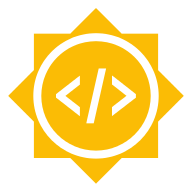
\includegraphics[width=0.25\textwidth]{pics/GSoC.png}
	\captionsource{The Google Summer of Code logo.}{\url{
        https://developers.google.com/open-source/gsoc/resources/marketing}}
	\label{fig:gsoc}
\end{figure}

%-----------------------------------------------------------------------------%
\section{Research Steps}
%-----------------------------------------------------------------------------%

The following steps were conducted for the research:

\begin{enumerate}
    \item Literature review \\
    This step focused on reading and understanding how the Django
    object-relational mapping (ORM) tool works, as well as JSON support on the
    database backends supported by Django. During this step, the underlying
    concepts of this research were studied in order to accomplish the research
    objectives.

    \item Experiments \\
    In this step, experiments were done by trying out existing JSONField
    implementations, which included the PostgreSQL implementation in Django,
    as well as third-party packages on the Python Package Index (PyPI). Some
    experiments were also done by modifying a third-party package to work
    better on different database backends.

    \item Implementation \\
    This step focused on the implementation of the JSONField model and form
    fields. This was initially done by copying the existing implementation
    from the django.contrib.postgres module to the django.db.models and
    django.forms modules. The tests for the existing implementation were also
    copied. From there, the work was to modify the JSONField implementation so
    that all tests could pass on all available database backends.

    After the JSONField implementation, this step was continued by implementing
    the data validation example and benchmarking. This included the creation of
    two small Django projects for demonstration purposes.

    \item Results Analysis \\
    In this step, the primary work was to document the different behaviors and
    support of the JSONField implementation on each database backend. This step
    also included analyzing the data validation and benchmarking
    implementations. For the benchmark, the analysis included comparing the
    performance of JSONField on all database backends.
\end{enumerate}

%-----------------------------------------------------------------------------%
\section{Report Structure}
%-----------------------------------------------------------------------------%

The structure of this report is as follows:

\begin{itemize}
    \item Chapter 1 \babSatu \\
        This chapter covers the background, problem definition, objectives,
        scope, position, and steps of this research.
    \item Chapter 2 \babDua \\
        This chapter covers the results of the literature review done prior to
        executing the research.
    \item Chapter 3 \babTiga \\
        This chapter covers the plan and problem analysis to prepare for the
        implementation.
    \item Chapter 4 \babEmpat \\
        This chapter covers the JSONField, the data validation example, and
        the benchmarking implementations.
    \item Chapter 5 \babLima \\
        This chapter covers the analysis of the implementation results. This
        also covers the comparison of the benchmarking results between the
        database backends.
    \item Chapter 6 \kesimpulan \\
        This chapter covers the conclusions of the research and some
        recommendations for further research.
\end{itemize}
